%#Split: 01_background  
%#PieceName: p01_background
% p01_background_00.tex
\KLBeginSubjectWithHeaderCommands{01}{2}{研究の位置づけ}{1}{F}{3}{\DCPDVeryFirstPageStyle}{\DCPDDefaultPageStyle}

\section{研究の位置づけ}
%    <<最大 1ページ>>

%s03_background
%begin 本研究の着想に至った経緯など ====================
\noindent [\textbf{研究計画の背景}]
%事例を持ってくる? 

近年、クラウドコンピューティングが普及している。これはクラウドベンダから計算資源をオンデマンドに借りる仕組みである。しかしこの仕組みは、\amikake{\textbf{クラウドベンダが攻撃者にならないという信用}}の元でのみ成り立つ。個人情報や営業秘密を含むプログラムなどを扱う場合、このような\amikake{\textbf{信用は前提とするべき}} \amikake{\textbf{でない}}。ベンダを信用しない場合、クラウドコンピューティングには2つの問題がある。\ref{prob:maliciousvender}データとプログラムがベンダに見えることと、\ref{prob:verifiability}実行結果がプログラムの出力だと保証できないことである。図1にこれらの問題をまとめた。これらは暗号学により解決可能\ref{paper:mktfhe}\ref{paper:boostVC}だが、都度の暗号化、復号を伴うため、\amikake{\textbf{オンプレミスのサーバと同様に扱える利便性}}が損なわれる。従って、これらの問題は\ref{prob:usability}利便性の維持をしたまま達成されなければならない。

 
\begin{figure}[h]
    \centering
    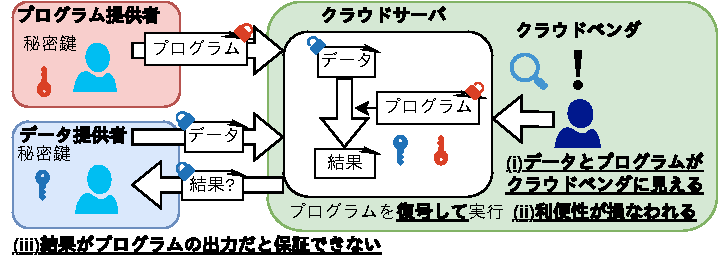
\includegraphics[width=0.8\linewidth]{figures/problem.drawio.pdf}
    \vspace*{-0.5cm}
    \caption{クラウドコンピューティングの問題点}
    \label{fig:my_label}
\end{figure}

\noindent[\textbf{課題・分野の状況}]
% 及びー
% 着想に至った経緯にまとめる
% 現状を書く
% ここ短くする
% 現状はいかにまとめる
\begin{enumerate}[label=(\roman*),leftmargin=0.5cm]
\setlength{\parskip}{0cm} % 段落間
\setlength{\itemsep}{0cm} % 項目間
% パラレルにする(利便性の維持を変更するか他を合わせる
    \item \underline{\textbf{データとプログラムがクラウドベンダに見える}}: 図1に示すように、クラウドコンピューティングではサーバ上でデータとプログラムは復号される。準同型暗号を用いれば暗号化したまま計算を行えるが、webサービスのようにプログラム提供者とデータ提供者が分かれる場合、計算量が鍵の本数の2乗に比例する[1]という問題がある。\label{prob:maliciousvender}
    \item  \underline{\textbf{実行結果がプログラムの出力だと保証できない}}: クラウドベンダはコストを抑えるため、プログラムを実行せず偽の結果を返す可能性がある。\amikake{\textbf{Verifiable Computation(VC)}}を用いれば結果がプログラムの実行結果であるかを検証できる。しかし、適用された準同型暗号が限られている[2]か、実装が存在しない[3]。\label{prob:verifiability}
    \item  \underline{\textbf{利便性の維持}}: 我々の過去の研究[4]では暗号化したままC言語を実行可能である。しかし、独自ISAを採用したためにコンパイラも独自であり、他の言語がサポートできていない。\label{prob:usability}
\end{enumerate}

\noindent[\textbf{着想に至った経緯}]
% 自身の前の研究を欠陥を指摘する感じに

準同型暗号を知った時、「これが論理関数(NAND)を計算できるのであれば、暗号のまま計算処理をするCPUが作れるはずだ」と考えた。本研究はこの発想を骨子として現代的コンピュータの進化形として構想した。

%end 本研究の着想に至った経緯など ====================

% p01_background_01.tex
\KLEndSubject{F}


